%% bare_jrnl.tex
%% V1.4b
%% 2015/08/26
%% by Michael Shell
%% see http://www.michaelshell.org/
%% for current contact information.
%%
%% This is a skeleton file demonstrating the use of IEEEtran.cls
%% (requires IEEEtran.cls version 1.8b or later) with an IEEE
%% journal paper.
%%
%% Support sites:
%% http://www.michaelshell.org/tex/ieeetran/
%% http://www.ctan.org/pkg/ieeetran
%% and
%% http://www.ieee.org/

%%*************************************************************************
%% Legal Notice:
%% This code is offered as-is without any warranty either expressed or
%% implied; without even the implied warranty of MERCHANTABILITY or
%% FITNESS FOR A PARTICULAR PURPOSE!
%% User assumes all risk.
%% In no event shall the IEEE or any contributor to this code be liable for
%% any damages or losses, including, but not limited to, incidental,
%% consequential, or any other damages, resulting from the use or misuse
%% of any information contained here.
%%
%% All comments are the opinions of their respective authors and are not
%% necessarily endorsed by the IEEE.
%%
%% This work is distributed under the LaTeX Project Public License (LPPL)
%% ( http://www.latex-project.org/ ) version 1.3, and may be freely used,
%% distributed and modified. A copy of the LPPL, version 1.3, is included
%% in the base LaTeX documentation of all distributions of LaTeX released
%% 2003/12/01 or later.
%% Retain all contribution notices and credits.
%% ** Modified files should be clearly indicated as such, including  **
%% ** renaming them and changing author support contact information. **
%%*************************************************************************


% *** Authors should verify (and, if needed, correct) their LaTeX system  ***
% *** with the testflow diagnostic prior to trusting their LaTeX platform ***
% *** with production work. The IEEE's font choices and paper sizes can   ***
% *** trigger bugs that do not appear when using other class files.       ***                          ***
% The testflow support page is at:
% http://www.michaelshell.org/tex/testflow/



\documentclass[journal]{IEEEtran}
%
% If IEEEtran.cls has not been installed into the LaTeX system files,
% manually specify the path to it like:
% \documentclass[journal]{../sty/IEEEtran}





% Some very useful LaTeX packages include:
% (uncomment the ones you want to load)

\usepackage{siunitx}
\usepackage{nicefrac}
\sisetup{
group-four-digits = true,
group-separator = {,}
}

% *** MISC UTILITY PACKAGES ***
%
%\usepackage{ifpdf}
% Heiko Oberdiek's ifpdf.sty is very useful if you need conditional
% compilation based on whether the output is pdf or dvi.
% usage:
% \ifpdf
%   % pdf code
% \else
%   % dvi code
% \fi
% The latest version of ifpdf.sty can be obtained from:
% http://www.ctan.org/pkg/ifpdf
% Also, note that IEEEtran.cls V1.7 and later provides a builtin
% \ifCLASSINFOpdf conditional that works the same way.
% When switching from latex to pdflatex and vice-versa, the compiler may
% have to be run twice to clear warning/error messages.






% *** CITATION PACKAGES ***
%
\usepackage{cite}
% cite.sty was written by Donald Arseneau
% V1.6 and later of IEEEtran pre-defines the format of the cite.sty package
% \cite{} output to follow that of the IEEE. Loading the cite package will
% result in citation numbers being automatically sorted and properly
% "compressed/ranged". e.g., [1], [9], [2], [7], [5], [6] without using
% cite.sty will become [1], [2], [5]--[7], [9] using cite.sty. cite.sty's
% \cite will automatically add leading space, if needed. Use cite.sty's
% noadjust option (cite.sty V3.8 and later) if you want to turn this off
% such as if a citation ever needs to be enclosed in parenthesis.
% cite.sty is already installed on most LaTeX systems. Be sure and use
% version 5.0 (2009-03-20) and later if using hyperref.sty.
% The latest version can be obtained at:
% http://www.ctan.org/pkg/cite
% The documentation is contained in the cite.sty file itself.






% *** GRAPHICS RELATED PACKAGES ***
%
\ifCLASSINFOpdf
  \usepackage[pdftex]{graphicx}
  %declare the path(s) where your graphic files are
  \graphicspath{{../pdf/}{../jpeg/}}
  %and their extensions so you won't have to specify these with
  %every instance of \includegraphics
  \DeclareGraphicsExtensions{.pdf,.jpeg,.png}
\else
  % or other class option (dvipsone, dvipdf, if not using dvips). graphicx
  % will default to the driver specified in the system graphics.cfg if no
  % driver is specified.
  % \usepackage[dvips]{graphicx}
  % declare the path(s) where your graphic files are
  % \graphicspath{{../eps/}}
  % and their extensions so you won't have to specify these with
  % every instance of \includegraphics
  % \DeclareGraphicsExtensions{.eps}
\fi
% graphicx was written by David Carlisle and Sebastian Rahtz. It is
% required if you want graphics, photos, etc. graphicx.sty is already
% installed on most LaTeX systems. The latest version and documentation
% can be obtained at:
% http://www.ctan.org/pkg/graphicx
% Another good source of documentation is "Using Imported Graphics in
% LaTeX2e" by Keith Reckdahl which can be found at:
% http://www.ctan.org/pkg/epslatex
%
% latex, and pdflatex in dvi mode, support graphics in encapsulated
% postscript (.eps) format. pdflatex in pdf mode supports graphics
% in .pdf, .jpeg, .png and .mps (metapost) formats. Users should ensure
% that all non-photo figures use a vector format (.eps, .pdf, .mps) and
% not a bitmapped formats (.jpeg, .png). The IEEE frowns on bitmapped formats
% which can result in "jaggedy"/blurry rendering of lines and letters as
% well as large increases in file sizes.
%
% You can find documentation about the pdfTeX application at:
% http://www.tug.org/applications/pdftex





% *** MATH PACKAGES ***
%
\usepackage{amsmath}
%\usepackage{newtxtext,newtxmath}
\usepackage{amssymb}
% A popular package from the American Mathematical Society that provides
% many useful and powerful commands for dealing with mathematics.
%
% Note that the amsmath package sets \interdisplaylinepenalty to 10000
% thus preventing page breaks from occurring within multiline equations. Use:
%\interdisplaylinepenalty=2500
% after loading amsmath to restore such page breaks as IEEEtran.cls normally
% does. amsmath.sty is already installed on most LaTeX systems. The latest
% version and documentation can be obtained at:
% http://www.ctan.org/pkg/amsmath





% *** SPECIALIZED LIST PACKAGES ***
%
%\usepackage{algorithmic}
% algorithmic.sty was written by Peter Williams and Rogerio Brito.
% This package provides an algorithmic environment fo describing algorithms.
% You can use the algorithmic environment in-text or within a figure
% environment to provide for a floating algorithm. Do NOT use the algorithm
% floating environment provided by algorithm.sty (by the same authors) or
% algorithm2e.sty (by Christophe Fiorio) as the IEEE does not use dedicated
% algorithm float types and packages that provide these will not provide
% correct IEEE style captions. The latest version and documentation of
% algorithmic.sty can be obtained at:
% http://www.ctan.org/pkg/algorithms
% Also of interest may be the (relatively newer and more customizable)
% algorithmicx.sty package by Szasz Janos:
% http://www.ctan.org/pkg/algorithmicx




% *** ALIGNMENT PACKAGES ***
%
%\usepackage{array}
% Frank Mittelbach's and David Carlisle's array.sty patches and improves
% the standard LaTeX2e array and tabular environments to provide better
% appearance and additional user controls. As the default LaTeX2e table
% generation code is lacking to the point of almost being broken with
% respect to the quality of the end results, all users are strongly
% advised to use an enhanced (at the very least that provided by array.sty)
% set of table tools. array.sty is already installed on most systems. The
% latest version and documentation can be obtained at:
% http://www.ctan.org/pkg/array


% IEEEtran contains the IEEEeqnarray family of commands that can be used to
% generate multiline equations as well as matrices, tables, etc., of high
% quality.




% *** SUBFIGURE PACKAGES ***
%\ifCLASSOPTIONcompsoc
%  \usepackage[caption=false,font=normalsize,labelfont=sf,textfont=sf]{subfig}
%\else
%  \usepackage[caption=false,font=footnotesize]{subfig}
%\fi
% subfig.sty, written by Steven Douglas Cochran, is the modern replacement
% for subfigure.sty, the latter of which is no longer maintained and is
% incompatible with some LaTeX packages including fixltx2e. However,
% subfig.sty requires and automatically loads Axel Sommerfeldt's caption.sty
% which will override IEEEtran.cls' handling of captions and this will result
% in non-IEEE style figure/table captions. To prevent this problem, be sure
% and invoke subfig.sty's "caption=false" package option (available since
% subfig.sty version 1.3, 2005/06/28) as this is will preserve IEEEtran.cls
% handling of captions.
% Note that the Computer Society format requires a larger sans serif font
% than the serif footnote size font used in traditional IEEE formatting
% and thus the need to invoke different subfig.sty package options depending
% on whether compsoc mode has been enabled.
%
% The latest version and documentation of subfig.sty can be obtained at:
% http://www.ctan.org/pkg/subfig




% *** FLOAT PACKAGES ***
%
%\usepackage{fixltx2e}
% fixltx2e, the successor to the earlier fix2col.sty, was written by
% Frank Mittelbach and David Carlisle. This package corrects a few problems
% in the LaTeX2e kernel, the most notable of which is that in current
% LaTeX2e releases, the ordering of single and double column floats is not
% guaranteed to be preserved. Thus, an unpatched LaTeX2e can allow a
% single column figure to be placed prior to an earlier double column
% figure.
% Be aware that LaTeX2e kernels dated 2015 and later have fixltx2e.sty's
% corrections already built into the system in which case a warning will
% be issued if an attempt is made to load fixltx2e.sty as it is no longer
% needed.
% The latest version and documentation can be found at:
% http://www.ctan.org/pkg/fixltx2e


%\usepackage{stfloats}
% stfloats.sty was written by Sigitas Tolusis. This package gives LaTeX2e
% the ability to do double column floats at the bottom of the page as well
% as the top. (e.g., "\begin{figure*}[!b]" is not normally possible in
% LaTeX2e). It also provides a command:
%\fnbelowfloat
% to enable the placement of footnotes below bottom floats (the standard
% LaTeX2e kernel puts them above bottom floats). This is an invasive package
% which rewrites many portions of the LaTeX2e float routines. It may not work
% with other packages that modify the LaTeX2e float routines. The latest
% version and documentation can be obtained at:
% http://www.ctan.org/pkg/stfloats
% Do not use the stfloats baselinefloat ability as the IEEE does not allow
% \baselineskip to stretch. Authors submitting work to the IEEE should note
% that the IEEE rarely uses double column equations and that authors should try
% to avoid such use. Do not be tempted to use the cuted.sty or midfloat.sty
% packages (also by Sigitas Tolusis) as the IEEE does not format its papers in
% such ways.
% Do not attempt to use stfloats with fixltx2e as they are incompatible.
% Instead, use Morten Hogholm'a dblfloatfix which combines the features
% of both fixltx2e and stfloats:
%
% \usepackage{dblfloatfix}
% The latest version can be found at:
% http://www.ctan.org/pkg/dblfloatfix




%\ifCLASSOPTIONcaptionsoff
%  \usepackage[nomarkers]{endfloat}
% \let\MYoriglatexcaption\caption
% \renewcommand{\caption}[2][\relax]{\MYoriglatexcaption[#2]{#2}}
%\fi
% endfloat.sty was written by James Darrell McCauley, Jeff Goldberg and
% Axel Sommerfeldt. This package may be useful when used in conjunction with
% IEEEtran.cls'  captionsoff option. Some IEEE journals/societies require that
% submissions have lists of figures/tables at the end of the paper and that
% figures/tables without any captions are placed on a page by themselves at
% the end of the document. If needed, the draftcls IEEEtran class option or
% \CLASSINPUTbaselinestretch interface can be used to increase the line
% spacing as well. Be sure and use the nomarkers option of endfloat to
% prevent endfloat from "marking" where the figures would have been placed
% in the text. The two hack lines of code above are a slight modification of
% that suggested by in the endfloat docs (section 8.4.1) to ensure that
% the full captions always appear in the list of figures/tables - even if
% the user used the short optional argument of \caption[]{}.
% IEEE papers do not typically make use of \caption[]'s optional argument,
% so this should not be an issue. A similar trick can be used to disable
% captions of packages such as subfig.sty that lack options to turn off
% the subcaptions:
% For subfig.sty:
% \let\MYorigsubfloat\subfloat
% \renewcommand{\subfloat}[2][\relax]{\MYorigsubfloat[]{#2}}
% However, the above trick will not work if both optional arguments of
% the \subfloat command are used. Furthermore, there needs to be a
% description of each subfigure *somewhere* and endfloat does not add
% subfigure captions to its list of figures. Thus, the best approach is to
% avoid the use of subfigure captions (many IEEE journals avoid them anyway)
% and instead reference/explain all the subfigures within the main caption.
% The latest version of endfloat.sty and its documentation can obtained at:
% http://www.ctan.org/pkg/endfloat
%
% The IEEEtran \ifCLASSOPTIONcaptionsoff conditional can also be used
% later in the document, say, to conditionally put the References on a
% page by themselves.




% *** PDF, URL AND HYPERLINK PACKAGES ***
%
\usepackage{url}
% url.sty was written by Donald Arseneau. It provides better support for
% handling and breaking URLs. url.sty is already installed on most LaTeX
% systems. The latest version and documentation can be obtained at:
% http://www.ctan.org/pkg/url
% Basically, \url{my_url_here}.




% *** Do not adjust lengths that control margins, column widths, etc. ***
% *** Do not use packages that alter fonts (such as pslatex).         ***
% There should be no need to do such things with IEEEtran.cls V1.6 and later.
% (Unless specifically asked to do so by the journal or conference you plan
% to submit to, of course. )


% correct bad hyphenation here
\hyphenation{op-tical net-works semi-conduc-tor}


\begin{document}

% this removes the url from biblio: Eurico Covas
\bstctlcite{IEEEexample:BSTcontrol}
% this removes the url from biblio: Eurico Covas

%
% paper title
% Titles are generally capitalized except for words such as a, an, and, as,
% at, but, by, for, in, nor, of, on, or, the, to and up, which are usually
% not capitalized unless they are the first or last word of the title.
% Linebreaks \\ can be used within to get better formatting as desired.
% Do not put math or special symbols in the title.
\title{Optimal Neural Network Feature Selection for Spatial-Temporal Forecasting}
%
%
% author names and IEEE memberships
% note positions of commas and nonbreaking spaces ( ~ ) LaTeX will not break
% a structure at a ~ so this keeps an author's name from being broken across
% two lines.
% use \thanks{} to gain access to the first footnote area
% a separate \thanks must be used for each paragraph as LaTeX2e's \thanks
% was not built to handle multiple paragraphs
%


% \author{Michael~Shell,~\IEEEmembership{Member,~IEEE,}
        % John~Doe,~\IEEEmembership{Fellow,~OSA,}
        % and~Jane~Doe,~\IEEEmembership{Life~Fellow,~IEEE}% <-this % stops a space
% \thanks{M. Shell was with the Department
% of Electrical and Computer Engineering, Georgia Institute of Technology, Atlanta,
% GA, 30332 USA e-mail: (see http://www.michaelshell.org/contact.html).}% <-this % stops a space
% \thanks{J. Doe and J. Doe are with Anonymous University.}% <-this % stops a space
% \thanks{Manuscript received April 19, 2005; revised August 26, 2015.}}

\author{Eurico~Covas,~\IEEEmembership{}
	    Emmanouil~Benetos~\IEEEmembership{}% <-this % stops a space
\thanks{E. Covas is with the CITEUC, Geophysical and Astronomical Observatory, University of Coimbra, 3040-004, Coimbra, Portugal, and
Queen Mary University London, 10 Godward Square, Mile End Rd, London E1 4FZ,  e-mail: (eurico.covas@mail.com)}% <-this % stops a space
\thanks{E. Benetos is with Queen Mary University London, 10 Godward Square, Mile End Rd, London E1 4FZ,
e-mail: (emmanouil.benetos@qmul.ac.uk)}% <-this % stops a space}\thanks{Manuscript received December 31, 2017; revised December 31, 2017.}
\thanks{Manuscript received x, 2018; revised xx, 2018.}}

% note the % following the last \IEEEmembership and also \thanks -
% these prevent an unwanted space from occurring between the last author name
% and the end of the author line. i.e., if you had this:
%
% \author{....lastname \thanks{...} \thanks{...} }
%                     ^------------^------------^----Do not want these spaces!
%
% a space would be appended to the last name and could cause every name on that
% line to be shifted left slightly. This is one of those "LaTeX things". For
% instance, "\textbf{A} \textbf{B}" will typeset as "A B" not "AB". To get
% "AB" then you have to do: "\textbf{A}\textbf{B}"
% \thanks is no different in this regard, so shield the last } of each \thanks
% that ends a line with a % and do not let a space in before the next \thanks.
% Spaces after \IEEEmembership other than the last one are OK (and needed) as
% you are supposed to have spaces between the names. For what it is worth,
% this is a minor point as most people would not even notice if the said evil
% space somehow managed to creep in.



% The paper headers
\markboth{}%
{Covas \MakeLowercase{\textit{et al.}}: Optimal Neural Network Feature Selection for Spatial-Temporal Forecasting}
% The only time the second header will appear is for the odd numbered pages
% after the title page when using the twoside option.
%
% *** Note that you probably will NOT want to include the author's ***
% *** name in the headers of peer review papers.                   ***
% You can use \ifCLASSOPTIONpeerreview for conditional compilation here if
% you desire.




% If you want to put a publisher's ID mark on the page you can do it like
% this:
%\IEEEpubid{0000--0000/00\$00.00~\copyright~2015 IEEE}
% Remember, if you use this you must call \IEEEpubidadjcol in the second
% column for its text to clear the IEEEpubid mark.



% use for special paper notices
%\IEEEspecialpapernotice{(Invited Paper)}




% make the title area
\maketitle

% As a general rule, do not put math, special symbols or citations
% in the abstract or keywords.
\begin{abstract}
We show empirical evidence on how to construct the optimal feature selection or input representation used by  
the input layer of a feedforward neural 
network for the propose of forecasting spatial-temporal signals. The approach is based on results from dynamical systems theory, namely 
the non-linear embedding theorems. We demonstrate it for a variety of spatial-temporal signals, with one spatial and one temporal 
dimensions, and show that the optimal input layer representation consists of a grid, with spatial/temporal lags determined by 
the minimum of the mutual information of the spatial/temporal signals and the number of points taken in space/time decided by the 
embedding dimension of the signal. We present evidence of this conjecture by running a Monte Carlo simulation of several combinations of 
input layer feature designs and show that the one predicted by the non-linear embedding theorems seems to be optimal or close of 
optimal. In total we show evidence in four unrelated systems: a series of coupled H\'{e}non maps; a series of couple Ordinary 
Differential Equations (Lorenz-96) phenomenologically modelling atmospheric dynamics; the Kuramoto-Sivashinsky equation, a partial
differential equation used in
studies of instabilities in laminar flame fronts and finally real physical 
data from sunspot areas in the Sun (in latitude and time) from 1874 to 2015.
\end{abstract}

% Note that keywords are not normally used for peerreview papers.
\begin{IEEEkeywords}
Neural network, Feedforward neural network, Input variables, Time series analysis, Forecasting, Prediction methods, Prediction algorithm,
Nonlinear system, Chaos, Spatiotemporal phenomena
\end{IEEEkeywords}






% For peer review papers, you can put extra information on the cover
% page as needed:
% \ifCLASSOPTIONpeerreview
% \begin{center} \bfseries EDICS Category: 3-BBND \end{center}
% \fi
%
% For peerreview papers, this IEEEtran command inserts a page break and
% creates the second title. It will be ignored for other modes.
\IEEEpeerreviewmaketitle



\section{Introduction}
% The very first letter is a 2 line initial drop letter followed
% by the rest of the first word in caps.
%
% form to use if the first word consists of a single letter:
% \IEEEPARstart{A}{demo} file is ....
%
% form to use if you need the single drop letter followed by
% normal text (unknown if ever used by the IEEE):
% \IEEEPARstart{A}{}demo file is ....
%
% Some journals put the first two words in caps:
% \IEEEPARstart{T}{his demo} file is ....
%
% Here we have the typical use of a "T" for an initial drop letter
% and "HIS" in caps to complete the first word.
\IEEEPARstart{G}{iven} a physical data set, one of the most important questions one can pose is: ``Can we predict the future ?'' This 
question can be put forward irrespectively of the fact that we may already have some insight or even be certain on what the exact model 
behind some or all the observed variables is. For example, for chaotic dynamical systems \cite{0813340853,2004icti.book.....M}, we may 
even have the underlying dynamics but still find it hard to predict the future, given that chaotic systems have exponential sensitivity 
to initial conditions. The more chaotic a system is (as measured by the positiveness of their largest Lyapunov exponents 
\cite{1985PhyD...16..285W,1994PhLA..185...77K}) the harder it gets to predict the future, even within very short time horizons. In the 
limit case of a random system, it is not possible to predict the future at all, although one can opine on certain future 
statistics\cite{9780486693873}. For the case of weakly chaotic systems, there is an extensive literature on forecasting methods ranging 
from linear approximations\cite{1451722}; truncated functional expansion 
series\cite{Powell:1987:RBF:48424.48433,Broomhead1988MultivariableFI}; non-linear embeddings \cite{PhysRevLett.59.845}; auto-regression 
methods\cite{0130607746}; hidden Markov models \cite{1165342} to state-of-the-art neural networks and deep learning methodologies 
\cite{LANGKVIST201411} and many others, too long to list here.

Most literature on forecasting chaotic signals is dedicated to a single time series, or treat a collection of related time series as a 
non-extended set, i.e. a multivariate set of discrete variables as opposed to a spatially continuous series. 
For forecasting spatial-temporal chaos we 
refer the reader to 
\cite{doi:10.1063/1.165894,PhysRevE.51.R2709,PhysRevLett.85.2300,ORSTAVIK1998145,
Parlitz2000NonlinearPO,2000PhRvL..84.1890P,Covas,Xia2006APF,ENV:ENV2266,covas2016,ENV:ENV2456} and 
references therein. Even rarer are attempts to forecast spatial-temporal chaos using neural networks and deep learning methodologies 
\cite{covaspeixinhojoao,2017arXiv170805094M,2017arXiv171100636M,2017arXiv171110566R,2017arXiv171110561R,2017arXiv171009668L, 
2017arXiv171205293C, ghaderi2017deepforecast,2017Chaos..27d1102L,
2018JCoPh.357..125R,2018arXiv180106637R}, although this field of research is clearly growing at the moment\footnote{
There is also a new emerging field of research on solving PDEs (therefore implicitly predicting a spatial-temporal
evolution) using deep learning -- see \cite{2017arXiv170905963B,2017arXiv170807469S,2017arXiv170604702E} and references therein.
Furthermore, notice that in this article we are concerned with the full space-time prediction, 
as opposed to the ongoing research on pattern recognition in moving 
images (2D and 3D), which attempt to pick particular features (e.g. car, pedestrian, bicycle, person, etc.) and to forecast where 
those features will be in subsequent images within a particular moving sequence -- see \cite{article_motion} and reference therein.
}.
 Nonetheless, this area of 
research is of importance, as most physical systems are spatially extended, e.g. the atmospheric system driving the Earth's weather
\cite{9780521857291}; the solar dynamo driving the Sun's sunspots \cite{9780198512905}; and the influence of sunspots on the Earth's 
magnetic field via the solar wind, coronal mass ejections and solar flares -- the so-called space weather 
\cite{1851RSPT..141..123S, 1852RSPT..142..103S, 1979P&SS...27.1001S,
1983SoPh...89..195E,1965P&SS...13....9P,2000AdSpR..26...27W,2003A&AT...22..861B,2005GeoRL..3221106S,
2005SpWea...3.8C01K,2006GMS...165..367T,2006GeoRL..3318101H, 2009SunGe...4...55C,2011SpWea...9.6001C,
2013EGUGA..1510865W}, which may have real economic implications \cite{2015SpWea..13..524S}.
Nonetheless its importance, forecasting spatial-temporal chaos is difficult.
The reasons are many, but mainly: first, the geometric dimension of the 
attractor \cite{1985PhLA..107..101G} -- usually quite large, the so-called curse of dimensionality \cite{9780486428093}; 
and second how to choose the variables to use for forecasting, i.e., is there 
enough information on the same point back in time to derive the future of that particular point, or do spatial correlations and spatial 
propagation affect it in a way that one must take into account some spatial and temporal neighbours set to forecast the future.
If this is the case, can that set of points be defined and how can it be constructed? 
It is this last question that we investigate in this article, in the 
particular context of spatial-temporal forecasting using neural networks. 

Feature extraction and the design of the input
representation of the 
input layer for a neural network is considered to be an art form, relying mostly on trial and error and domain knowledge (see \cite{5771385}
for examples and references). For 
forecasting of time series, a simple approach consists of designing the input layer as a vector of previous data using a time delay, the 
time delay neural network method \cite{Waibel:1990:PRU:108235.108263, luk2000study, 857903, Frank2001, OH2002249, 1009-1963-12-6-304, 
inputlayer}. For spatial-temporal series, one can generalize it to include temporal and spatial delays 
\cite{covas2016,covaspeixinhojoao}. This is where the connection to dynamical systems can be useful. In 1981, Takens established the 
theoretical background \cite{1981LNM...898..366T} in his embedding theorem for a mathematical method to reconstruct the dynamics 
of the underlying attractor of a chaotic dynamical system from a time ordered sequence of data observations. Notice the reconstruction 
conserves the properties of the original dynamical system up to a diffeomorphism. 
 Further developments established a series of theorems \cite{key1503303m, 1981LNM...898..230M, 1991JSP....65..579S}
 that provided the basis for a non-linear embedding and forecasting on the original variables. The 
theorems and related articles propose to use a time delay approach with the time lag based on the first minima of the 
{\em mutual information}\footnote{
Notice that another non-linear dynamical systems technique exists to calculate this time delay, the zero of the autocorrelation
function \cite{opac-b1092652,abarbanel1997analysis}, but essentially these two approaches are after the same objective, i.e.
to select uncorrelated 
 variables as much as possible for optimal reconstruction embedding. So, in this article, we focus only on the first minima
 of the mutual information for simplicity of analysis.
} -- see 
\cite{Fraser86, abarbanel1997analysis, opac-b1092652} -- and to choose the number of points to include using  the method of {\em false 
nearest neighbours} detection suggested by \cite{1992PhRvA..45.3403K} and reported in detail in \cite{1992PhRvA..45.7058M, 
1993RvMP...65.1331A, 1996PhT....49k..86A, abarbanel1997analysis}. Using this theoretical framework, we conjecture that this non-linear 
embedding method can be used to indicate what the best way to construct the feature representation for 
the input layer of a neural network used for forecasting both in space and time.
In order to support this conjecture, we, in this article, show empirical evidence for an optimal feature selection 
 for four particular cases of a two-dimensional
spatial-temporal data series $s^n_m$, where by two-dimensional we mean a scalar field that can be
defined by a $N \times M$ matrix with components $s^n_m \in \mathbb{R}$.

Some authors discuss the use of either the mutual information and/or embedding dimension as a constraint on feature representation
\cite{annunziato, Gkana201579, Zachilas2015, Sun2010109, HUANG20108590, 298224, Frank2001, 1998GeoRL..25..457K, 
BUHAMRA2003805, chandra2012cooperative, DBLP:journals/corr/MaslennikovaB14, sauter2010spatio, JiangS11, inputlayer, 1997IJMPC...8.1345K, 
1009-1963-12-6-304, Verdes2000, 1996SoPh..168..423F, 2007AdG....10...67L, Chandra:2012:CCE:2181341.2181747, raios, 
maass2003mathematical,0305-4470-28-12-012, 1995ApJ...444..916C, 1998GeoRL..25..457K, Zachilas2015, Chandra:2012:CCE:2181341.2181747, 
Gkana201579, raios}. Others \cite{Simon:2007:HDS:1230147.1230294} attempted to generalize the mutual 
information approach to higher dimensions but do not actually connect it to the problem of spatial-temporal forecasting using neural networks. 
There are also authors \cite{articleRagulskis} that try to use neural networks to determine the optimal embedding and time 
delay for the purpose of local reconstruction of states with a view to forecast (the opposite of what we try to empirically demonstrate 
here). Fig.\ 6 in \cite{1555956} shows how the forecasting error for a pure time series prediction changes with the delay and the number of 
time delay points used as an input -- they use a reinforcement learning based dimension and delay estimator to derive the best dimension 
and delay, but do not seem to show that it is the dynamical systems derived values that are indeed optimal for forecasting neither
they show any extension to spatial-temporal signals as we demonstrate in this article.
Other authors \cite{Xia2006APF} try to use Support Vector Machines (SVMs) to forecast spatial-temporal signals and use delays and 
embedding approaches to define the states vectors. In fact, Parlitz and Merkwirth \cite{Parlitz2000NonlinearPO} in their
ESANN (European Symposium on Artificial Neural Networks) 2000 meeting proceedings' article mention
 that local reconstruction of states ``\ldots may also serve as
a starting point for deriving local mathematical models in terms of polynomials,
radial basis functions or neural networks\ldots''. Here we attempt to show empirical evidence that this is not just
a starting point, but the optimal neural network input feature selection. We also emphasise that,
 as far as we are aware, all the references on neural network forecasting of spatial-temporal dynamics that use the 
embedding theorems and the related mutual information and the false nearest neighbours methods seem not to justify its use, i.e., 
the approach is explained, even suggested to be optimal but neither proven theoretically or empirically. Here we attempt 
to provide an empirical evidence for this optimality. 
 
The article is divided as follows, in section \ref{modelsection} we explain our forecasting model, in section \ref{conjecturesection} 
we propose our conjecture, in section \ref{resultssection} we show our results supporting this conjecture and finally in section
\ref{conclusionsection} we make our concluding remarks.
\\

\hfill Eurico Covas and Emmanouil Benetos

\hfill \today

\section{The model}
\label{modelsection}

The neural network architecture we choose to demonstrate our possible conjecture is a form of the basic feedforward neural network,
sometimes called the time-delayed neural network \cite{Waibel:1990:PRU:108235.108263}, trained using the so-called back-propagation
algorithm \cite{10.1007/BFb0006203, 1986Natur.323..533R, 58337, Lecun98gradient-basedlearning}. 
We focus on spatial-temporal series, so we have extended the usual time-delayed neural network
to be a time and space delayed network. The overall feature representation of the network is depicted in detail in Fig.\ 
\ref{architecture}.

% to edit do the following 3 commands
% inkscape architecture.svg (then print to architecture.pdf)
% pdf270 --suffix 'turned' --batch architecture.pdf
% pdfcrop architecture-turned.pdf
\begin{figure}[!htb]
\resizebox{\hsize}{!}{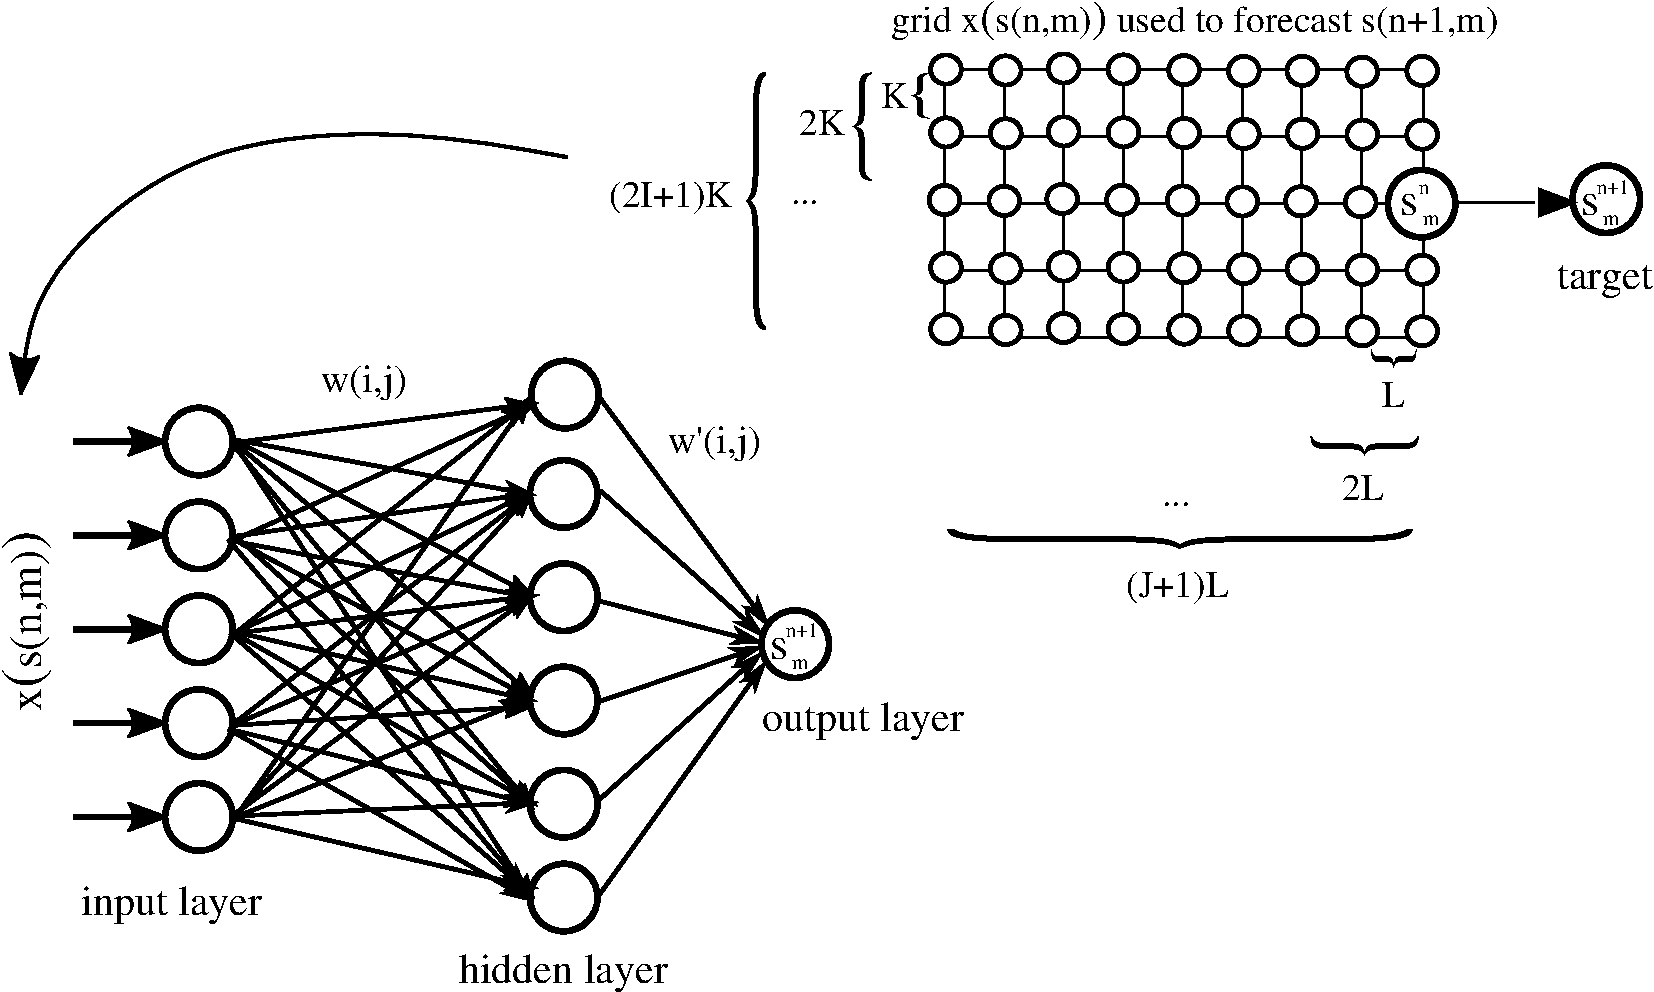
\includegraphics{architecture-turned-crop.pdf}}
\caption{Neural network architecture for forecasting spatial-temporal signals. 
The neural network is made of an input layer, one or more hidden layer(s) and one output layer.
In this article, for simplicity, we use only one hidden layer and the output layer is made of a single neuron. 
Each input pattern $x(i)$ is sent to the
input layer, then each of the hidden neurons values is calculated from the sum of the product of the weights by the inputs $\sum w(i,j) x(i)$
and passed via the non-linear activation function. Then the output is calculated by the product of the second set of
weights times the hidden node values $\sum w'(i,j) y(i)$ again passed to another (or the same) activation function.
Each input pattern $x(i)$ is actually a matrix constructed using an embedding space of
spatial and temporal delays, calculated from the actual physical spatial-temporal data values $s(n,m)$. After many randomly chosen input patterns
are passed via the neural network, the weights hopefully converge to an optimal training value. One can then forecast using the last
time slices of the training set, and compare against the test set, the real future data set.}
\label{architecture}
\end{figure}

Under this input representation, we use the ideas proposed in \cite{Parlitz2000NonlinearPO, 2000PhRvL..84.1890P} to construct a grid of input values
which are then fed to the neural network to produce a single output, the future state. Formally,
let $n=1,...,N$ and $m=1,...,M$.
Consider a spatial-temporal data series ${\bf s}$ which can be
defined by a $N\times M$ matrix with components
$s^n_m \in \mathbb{R}$. To these components, we will call {\em states} of the spatial-temporal series.
Consider a number $2I\in \mathbb{N}$ of neighbours in space of a given
$s^n_m$ and a number $J\in \mathbb{N}$ of temporal past neighbours relative to $s^n_m$ (see Fig.\ \ref{architecture} for details).
For each $s^n_m$, we define the input (feature) vector ${\bf x} (s^n_m)$ with components given by
$s^n_m$, its $2I$ spatial neighbours and its $J$ past temporal
neighbours, and with $K$ and $L$ being the spatial and temporal lags:
\begin{IEEEeqnarray}{rCl}
\label{embedding}
{\bf x}(s^n_m)&=&\{s^n_{m-I K }, ...,s^n_m, ..., s^n_{m+I K},\\
&& {}s^{n-L}_{m-I K},..., s^{n-L}_{m},..., s^{n-L}_{m+I K},
\ldots \nonumber\\ 
&& {}\ldots,s^{n-J L}_{m-I K},..., s^{n-J L}_{m},..., s^{n-J L}_{m+I K} \}
\nonumber
\end{IEEEeqnarray}

So, the input is a
$(2 I+1)(J+1)$ vector ${\bf x}(s^n_m)$ and the target (output) to train the network is the value $s^{n+1}_{m}$.
 We train the network using stochastic gradient
back-propagation by running a stochastic batch
where we randomly sample pairs of inputs and outputs from the training set: ${\bf x}(s^n_m)$ and $s^{n+1}_{m}$, respectively. Then at test time
we choose inputs ${\bf x}(s^n_m)$, such that $n=N_{train}$, $N_{train}$ being the number of temporal slices on the training set.
As for the remaining architecture, we use one hidden layer with $N_h$ nodes.
Regarding the back-propagation hyperparameters, we included an adaptive learning rate $\eta_n=\eta/(1+n/10000)$, 
where the hyperparameter $\eta$ is the initial learning rate and $\eta_n$ is the learning rate used at time step
$n$. We included a momentum $\alpha$ for faster convergence.
 A further hyperparameter is the choice of the activation function (see \cite{9780262527019}), we use either a ReLu (rectified linear unit)
 or a logistic sigmoid function depending on the
 test case we are working with.
We also normalize the data before passing it through the neural network, in most cases we scale it in linear fashion
$x \to \alpha_{nor} + x/\beta_{nor}$, and in the case of real physical data as we will see later, 
we scale it in logarithmic fashion it by $x \to \alpha_{nor}+\nicefrac{\ln(1+x)}{\beta_{nor}}$, where $x$ is the initial data,
and $\alpha_{nor}$ and $\beta_{nor}$ are the arbitrary shift and scaling constants, respectively. For the weight (and bias)
initialization we choose random numbers with a constant distribution between $[0,1]$ and shifted by $\alpha_{rng}$ and scaled
by $\beta_{rng}$. The final hyperparameter is the number of epochs taken on the stochastic gradient descent
which we denote by $N_{\textnormal{steps}}$.  
All of these hyperparameters are calibrated and fixed
before we do any simulations with respect to the parameters $I$, $J$, $K$, $L$, which are auto-calibrated by the above mentioned
methods derived from dynamical systems theory. In this sense, $I$, $J$, $K$, $L$ are not hyperparameters of the neural network. We use the standard
loss function $\mathcal{L}=\left( s^{n+1}_{m} - \hat{s}^{n+1}_{m}\right)^2$ for a prediction $\hat{s}^{n+1}_{m}$ 
centred around $s^{n}_{m}$ using as input
the features vector ${\bf x}(s^n_m)$ of total dimension  $(2 I+1)(J+1)$.




\section{Conjecture}
\label{conjecturesection}

\begin{figure}[!htb]
\resizebox{\hsize}{!}{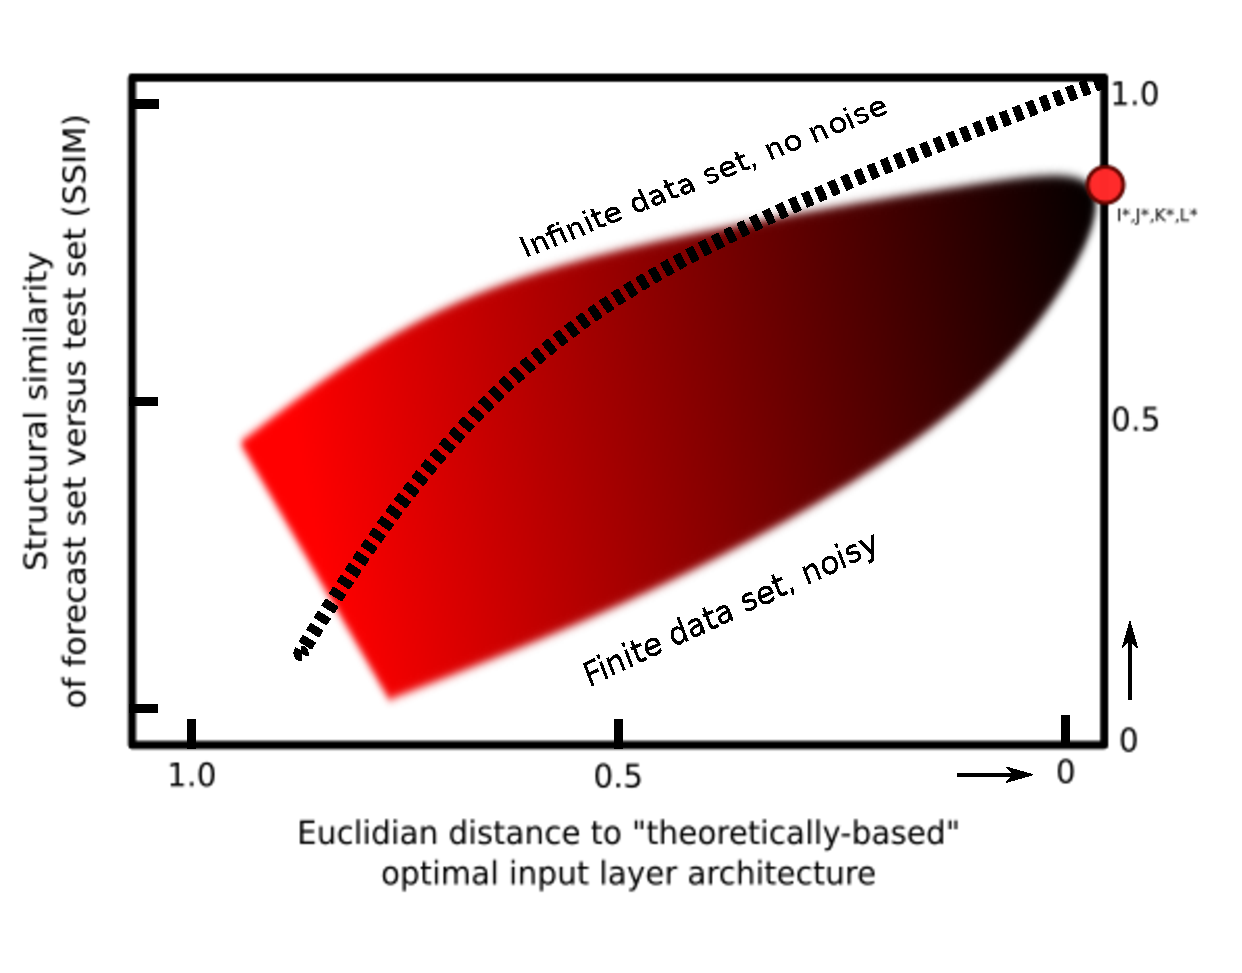
\includegraphics{conjecture-crop.pdf}}
\caption{Our main conjecture. For a infinite noiseless training set, the SSIM approaches $\textnormal{SSIM} \to 1$. For real data sets,
there is a dispersion of the SSIM versus some reasonable metric constructed to
 represent the distance between any feature selection (e.g.\ $d_e\sqrt{(I-I^*)^2+(J-J^*)^2+(K-K^*)^2+(L-L^*)^2}$).
}
\label{conjecture}
\end{figure}

Once we do a forecast, we then compare the goodness of fit by first visual inspection and second by numerically calculating the so-called
structural similarity $\textnormal{SSIM}(x,y)$ which has been proposed by \cite{Wang04imagequality} and used already in the context of spatial-temporal forecasting in \cite{covas2016, covaspeixinhojoao}. It has also been used in the context of deep learning used for enhancing
resolution on two dimensional images \cite{2015arXiv150100092D} and restoring missing data in images \cite{2018arXiv180208369Z}. For details on the SSIM measure see \cite{Wang04imagequality,2009ISPM...26...98W, 2012ITIP...21.1488B}.
The SSIM index is a metric quantity used to calculate the perceived quality of digital images and videos.  It
allows two images to be compared and provides a value of their similarity - a value of $\textnormal{SSIM}=1$ corresponds to the case of two
perfectly identical images. We use it by calculating the $\textnormal{SSIM}(x,y)$ between the entire test set and the forecast set,
since these can be interpreted as images (one spatial dimension/one temporal dimension).



Here we propose that the optimal time delay/spatial delays ($L$ and $K$, respectively) must be the ones based on the first minima of the mutual 
information \cite{Fraser86, abarbanel1997analysis, opac-b1092652} and that the optimal number of temporal/spatial points to use ($J$ and $I$, 
respectively) must be the ones based on the  the method of method of false nearest neighbours detection \cite{1992PhRvA..45.3403K, 
1992PhRvA..45.7058M, 1993RvMP...65.1331A, 1996PhT....49k..86A, abarbanel1997analysis}.  The mutual information is calculated by taking a $s^{i}$, a 
one-dimensional data set, and $s^{i+L}$, the related $L$-lagged data set. Given a measurement $s^i$, the amount of information $I(L)$ is the number 
of bits on $s^{i+L}$, on average, that can be predicted. We then average over space and take the first minimum of $\langle I(L) \rangle$, or, in the 
absense of a clear minimum, take the $L$ temporal lag for which the $\langle I(L) \rangle$ drops significantly and starts to plateau. This calculates 
$L^*$, the optimal time delay. Conversely, we calculate $K^*$ by calculating the spatial lag $K$ for which we obtain the first minima of the 
time-averaged mutual information $\langle I(K) \rangle$. Once the optimal spatial and temporal lags $K^*$ and $L^*$ are calculated, we calibrate 
the minimum embedding dimension, or in other words, the number of spatial and temporal neighbours in optimal  
phase space reconstruction. We use the method of false neighbours \cite{1992PhRvA..45.3403K, 1992PhRvA..45.7058M,1993RvMP...65.1331A},
which determines that falsely apparent close neighbours have been 
eliminated by virtue of projecting the full orbit in a increasing higher dimensional embedding phase space. This gives us the 
$J^*$, the optimal number of time slices to take,
and $I^*$, the optimal number of spatial slices to take in our ${\bf x}(s^n_m)$ optimal reconstruction.

In this article, we conjecture that as any set of input representation 
``approaches'' the optimal one, then $\textnormal{SSIM} \to 1$. In the case of finite training sets and/or noisy training sets  
$\textnormal{SSIM} \to x<1$, where $x$ is the best forecast possible given the data set. Visually, we believe that the SSIM versus some reasonable 
metric constructed to represent the distance between any input representation and the optimal input representation will show a skewed bell shape 
as depicted in Fig.\ \ref{conjecture}. In this conjecture, we use the most obvious candidate to represent the distance between any input 
representation and the optimal   input representation, the Euclidian distance given by   
$d_e=\sqrt{(I-I^*)^2+(J-J^*)^2+(K-K^*)^2+(L-L^*)^2}$, where $I$,$J$,$K$,$L$ are the parameters for each representation
and $I^*$,$J^*$,$K^*$,$L^*$ are the ones derived from the dynamical systems theory. We also verified that other reasonable metrics,   
in particular the Manhattan distance\cite{0486252027}, did 
not change the results qualitatively.
 








% needed in second column of first page if using \IEEEpubid
%\IEEEpubidadjcol

\section{Results}
\label{resultssection}

In order to empirically substantiate our conjecture, we take four examples of spatial-temporal series and attempt
to forecast using our feedforward neural network. 
First, we calculate the optimal time delay/spatial delays ($L^*$ and $K^*$, respectively)
using the first minima of the mutual information, then we calculate the optimal number of temporal/spatial points to use
($J^*$ and $I^*$, respectively) using the method of false nearest neighbours.
We then use a Monte Carlo simulation on each one of our four examples, sampling random values
of the key feature selection parameters: $I$, $J$, $K$, $L$ (including the trivial ones with $I=0$ and/or $J=0$) 
and calculate the values $d_e(I,J,K,L)$ 
and $\textnormal{SSIM}(I,J,K,L)$.
We plot the latter as a function of the former to compare against our conjecture as depicted in Fig.\ \ref{conjecture}.

We first take a physical system example, a real data example, and then we progress from ``simpler'' systems (coupled maps) 
capable of generating 
spatial-temporal chaos to more ``complex'' systems (coupled Ordinary Differential Equations - ODEs) to really ``complex'' systems (Partial 
Differential Equations - PDEs). This is partially motivated by results in the literature that show that general universalities are 
present in different levels of simplification of physical models \cite{2001Chaos..11..404C}, 
from the original PDEs to truncated ODE expansions (e.g. spectral 
method expansions \cite{2001cfsm.book.....B}) to the most extreme simplification or discretization such as maps 
which capture the essence of the problem(s). In all cases we take examples with one spatial and one temporal dimension. 
However, we believe 
that our conjecture will extend to multiple spatial dimensions. Notice that here we are not trying to demonstrate
that neural networks, and in particular feedforward neural networks can perform well in predicting spatial-temporal chaos
(as this has been demonstrated in the literature already), but 
rather to show that the optimal choice of the input layer features is given by dynamical systems theory and does not need to be
another neural network hyperparameter calculated by the ``dark art'' of trial and error.

\subsection{Sunspot data - a physical system example}

% code and results in
% C:\Users\eurico\SunspotAnalysis\NeuralNetworks\SolarForecastingNeuralNetworks41.xlsm

\begin{figure}[!htb]
\centering
\resizebox{\hsize}{!}{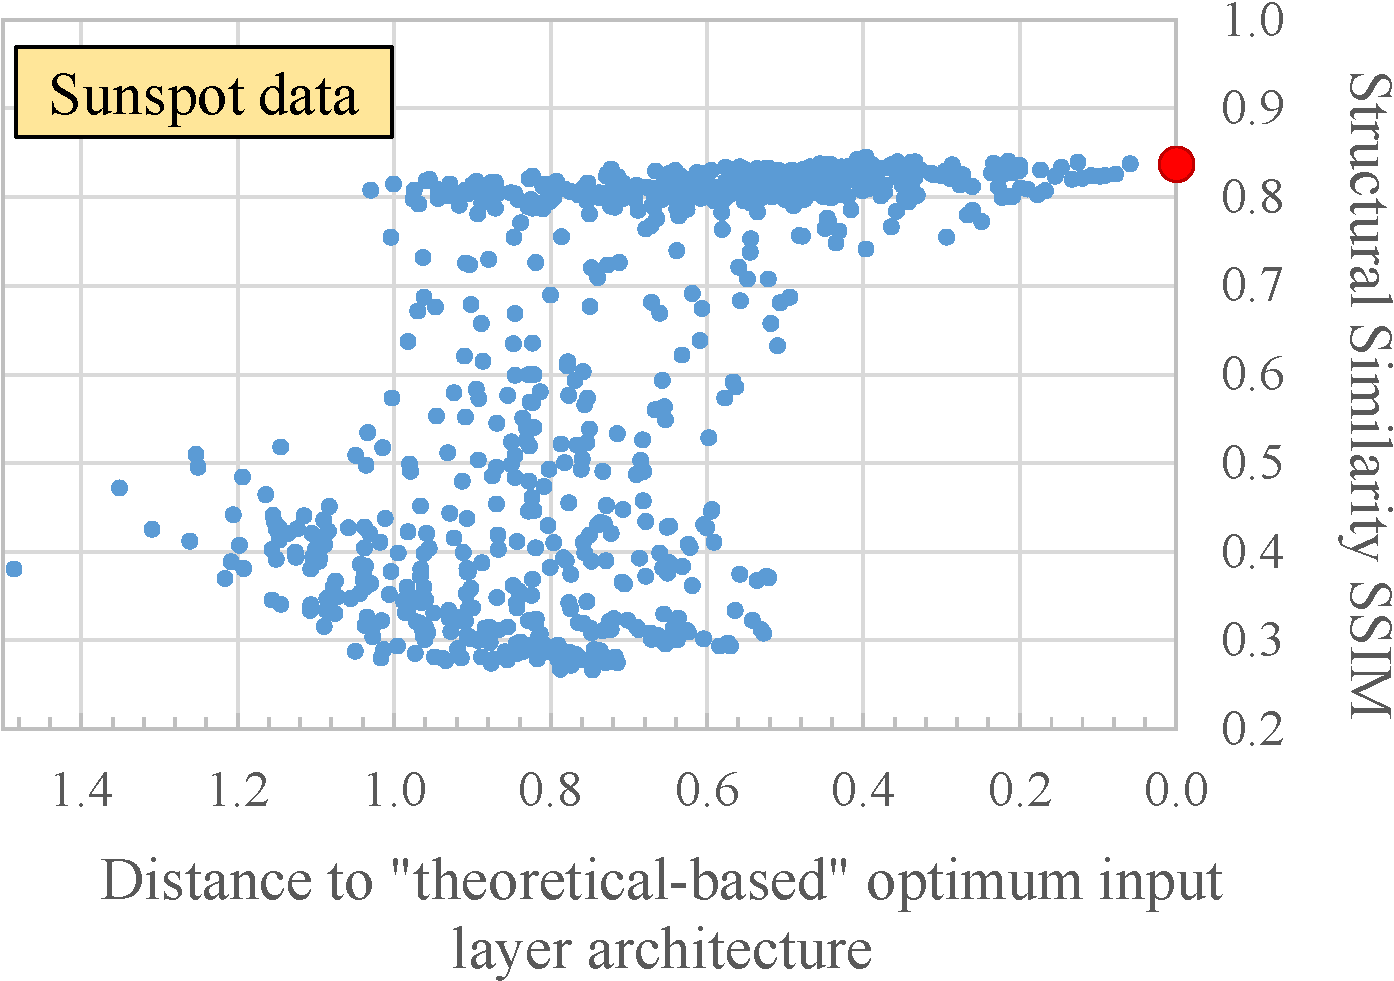
\includegraphics[]{MonteCarloSSIMversusParameterMetricDistance-crop.pdf}}
\caption{Monte Carlo simulation of different  input representations  of the input layer for the neural network forecast for the sunspot data.
It shows the structural similarity (SSIM) against how far (in a Euclidean space metric) the particular parameters of a particular
run were from the supposedly optimal input representation parameters (red dot).}
\label{MonteCarloSSIMversusParameterMetricDistance}
\end{figure}

The first example we take is a physical real data example based on a previous article of one of us \cite{covaspeixinhojoao}, where a 
neural network using the type of input representation above (Fig.\ \ref{architecture}) was used to forecast sunspot areas $A(t,\theta)$ in our 
Sun in both space ($\theta$ latitude) and time (Carrington Rotation index\footnote{Given that the surface solar rotation 
varies with time and latitude,
any approach of comparing positions on the Sun over a period of time is necessarily subjective.
Therefore, solar rotation is arbitrarily taken to be 27.2752316 days
for the purpose of Carrington rotations. Each solar rotation is given a 
number, the so-called Carrington Rotation Number, starting from 9th November, 1853.}). This sunspot data is usually called the
``butterfly diagram'' due to its butterfly wings like appearance \cite{1904MNRAS..64..747M}. One can see how this butterfly diagram looks like in
\cite{BibEntry2018Mar}.

Sunspot data is regularly seen as a benchmark for time series forecasting, given its chaotic nature and that it considered to be among the 
longest continuously recorded daily measurement made in science \cite{2013Natur.495..300O}.
Many authors \cite{
1990EOSTr..71..677K,
1991PhDT.......158W,
Weigend92HubermanRumelhart,
1993AdSpR..13..447M,
1995JGR...10021735M,
1994VA.....38..351C,
0305-4470-28-12-012,
1995ApJ...444..916C,
Koskela96timeseries,
1996SoPh..168..423F,
1996AnGeo..14...20F,
1996ITNN....7..501P,
1998GeoRL..25..457K,
1998JGR...10329733C,
1998NewAR..42..343C,
Verdes2000,
2004SoPh..221..167V,
2001GMS...125..201L,
2002PhRvE..66f6701S,
2004SoPh..224..247M,
2005JASTP..67..595G,
2004SPIE.5497..542A ,
2005MmSAI..76.1030Q,
2005SoPh..227..177A,
2006JASTP..68.2061M,
2007SoPh..243..253Q ,
2013Ap&SS.344....5A,
xie2006hybrid,
2006SunGe...1a...8M,
2007IJMPC..18.1839E,
1997SPIE.3077..116P,
2006AGUFMSH21A0315L,
2008cosp...37.3467W,
gang2007sunspot,
2009JASTP..71..569U,
2010BAAA...53..241F,
1999BAAA...43...23P,
2011RAA....11..491A,
2010cosp...38.2153A,
2011CRGeo.343..433C,
JiangS11,
2012cosp...39.1194M,
Chandra:2012:CCE:2181341.2181747,
park2009prediction ,
kim2010sunspot,
moghaddam2013sunspot,
2012EPJP..127...43C,
liu2012sunspot,
Gkana201579,
DBLP:conf/ijcnn/ParsapoorBS15,
DBLP:conf/aaai/ParsapoorBS15,
raios
} have already attempted to use neural networks to forecast aspects of the sunspot cycle, although as far as we are aware, 
none in both space and time having 
restricted themselves to using these neural networks to forecast mostly either the sunspot number or the sunspot areas as a function of 
time.  There is only one example\cite{covaspeixinhojoao}, as far as we are aware, of actual spatial-temporal forecasts using neural networks (see also 
\cite{2006AGUFMSH21A0315L,2008cosp...37.3467W} where a neural network forecast of the magnetic flux, which is related to sunspots, is forecast
for latitude/longitude datasets). There are also a few examples of forecasting the butterfly diagram sunspot data in both space and time (latitude/time)
\cite{2011A&A...528A..82J, 2016ApJ...823L..22C, 0004-637X-792-1-12, 2017arXiv170700268J, covas2016, 2017arXiv171207501S} but none of these used neural networks, rather
all of those used other statistical methods or numerical physical modelling.


We take as a ``training set'' the data from the year 1874 to 
approximately 1997 (i.e.\ the first 1646 Carrington Rotations). We then attempt to reproduce or forecast the sunspot area butterfly 
diagram from Carrington Rotation 1921 up to 2162 (the last one corresponding approximately to the year 2015); that is, we use 1646 time 
slices ($\approx 122.92$ years) to reproduce the next 242 time slices ($\approx 18.07$ years)\footnote{We use exactly
the same training set/forecast set slicing as in \cite{covas2016,covaspeixinhojoao} for consistency, even if more data is already
available at this time.}. The training set 
corresponds to around 12 solar cycles (cycle 11 to 22), while the ``forecasting set'' equates to around 1.5 cycles 
(cycle 23 and half of cycle 24). The entire dataset, including the training and forecasting sets, is a grid $x^i_j=x(i,j)$, with 
$i=1888$ and $j=50$. The training set is a grid $x(1646,50)$. For this case the optimal values were $I^*=2$, $J^*=6$, $K^*=9$ and 
$L^*=70$ as calculated in \cite{covas2016}. 
The hyperparameters of the neural network were:
$N_h=70$, $\eta=0.3$, $\alpha=0.01$, a logarithmic normalization of the inputs scaled
 with $\alpha_{nor} = 10$ and $\beta_{nor} = 0$, weight initialization with $\alpha_{rng} = 10^{-2}$ and $\beta_{rng} = -0.5$ 
 and $N_{\textnormal{steps}}=$\SI{1000000}\nobreak. We used the logistic sigmoid function as the activation on both the hidden and output layers.

The Monte Carlo results are depicted in Fig.\ \ref{MonteCarloSSIMversusParameterMetricDistance} showing runs with different $I$, $J$, $K$, $L$
and plotting the SSIM versus the distance to the optimal input feature selection parameters ($I^*$,$J^*$,$K^*$,$L^*$) 
given by the dynamical systems theory.  
It shows a reasonable expected dispersion as conjectured and 
a good convergence to the highest $\textnormal{SSIM}$ value we could obtain for this particular slicing of the training and forecast sets 
$\textnormal{SSIM}= 0.836876152$. From the figure, there seems to be also two clusters of behaviour, and at closer inspection, we found that the
cluster with lower SSIM is basically a set of very bad forecasts, with none of the characteristics of the real sunspot behaviour (the 11 year-like cycle
and the migration to the latitudinal equator), while the higher SSIM cluster corresponds to visually recognizable sunspot butterfly-like diagrams.



These results were quite satisfactory and inspired us to attempt to check the existence of a universality of behaviour across
dynamical systems, by examining other unrelated synthetic
generated data sets. We continue below to these attempts.


% An example of a floating figure using the graphicx package.
% Note that \label must occur AFTER (or within) \caption.
% For figures, \caption should occur after the \includegraphics.
% Note that IEEEtran v1.7 and later has special internal code that
% is designed to preserve the operation of \label within \caption
% even when the captionsoff option is in effect. However, because
% of issues like this, it may be the safest practice to put all your
% \label just after \caption rather than within \caption{}.
%
% Reminder: the "draftcls" or "draftclsnofoot", not "draft", class
% option should be used if it is desired that the figures are to be
% displayed while in draft mode.
%


\subsection{Coupled H\'{e}non maps - a discrete-time dynamical system}

\begin{figure}[!htb]
\centering
\resizebox{\hsize}{!}{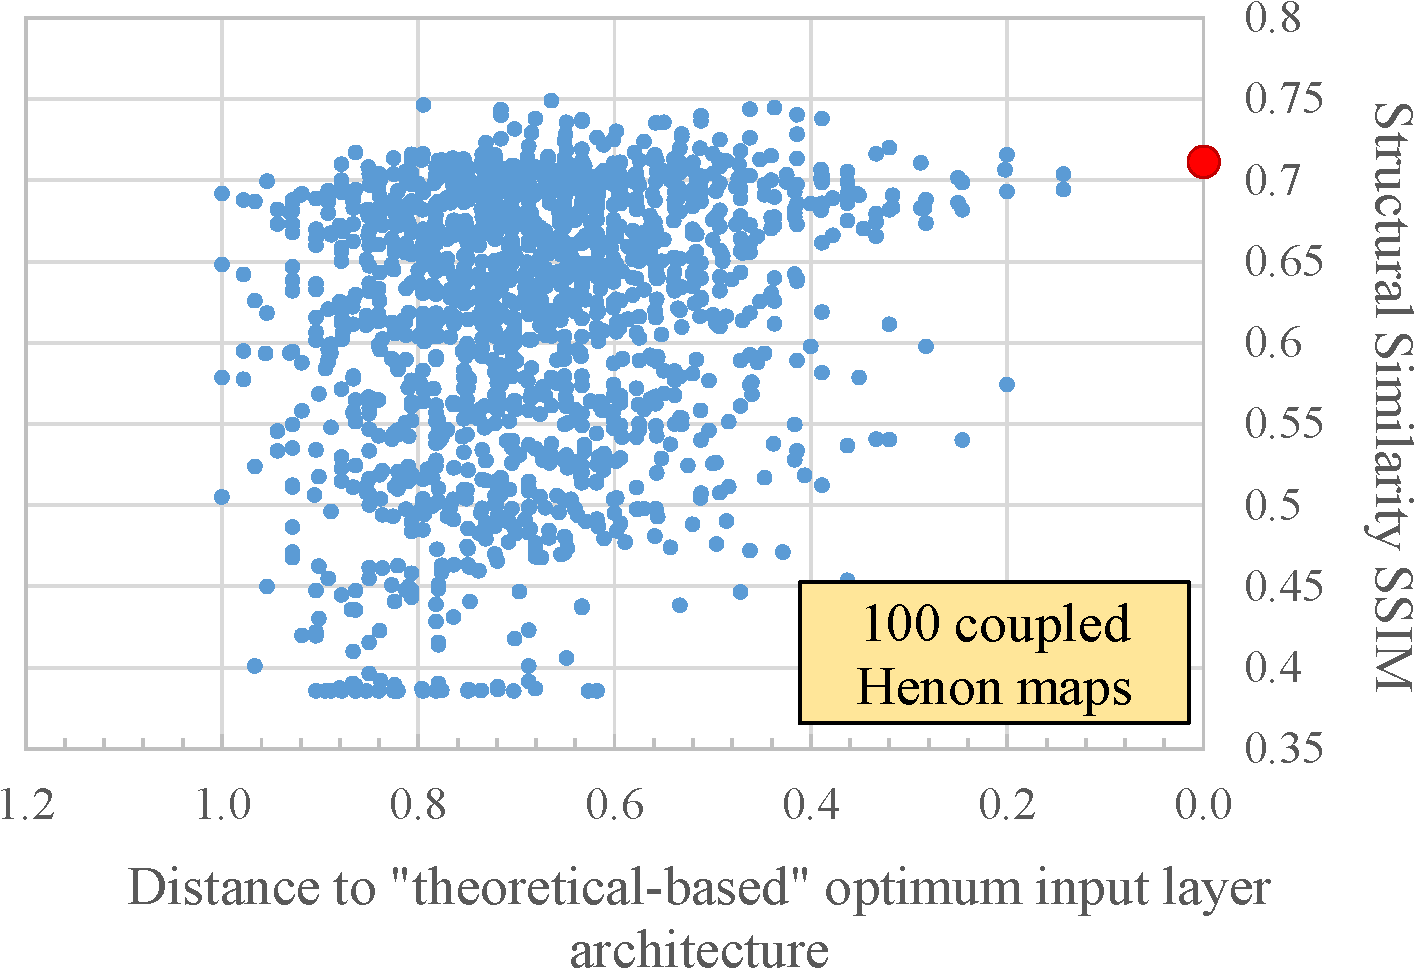
\includegraphics[]{MonteCarloSSIMversusParameterMetricDistance100HenonCoupledMaps-crop.pdf}}
\caption{Monte Carlo simulation of different  input representations of the input layer for the neural network forecast for a series of 100 coupled
H\'{e}non maps.
It shows the structural similarity (SSIM) against how far (in a Euclidean space metric) the particular parameters of a particular
run was from the supposedly optimal input representation parameters (red dot). The green line (trendline) seems to show that as the parameters
of a randomly chosen input representation get close to the supposedly optimal input representation ones, the SSIM converges to what seems to be the
best possible forecast value given the limited dataset.}
\label{MonteCarloSSIMversusParameterMetricDistance100HenonCoupledMaps}
\end{figure}

% code and results in
% C:\Users\eurico\SunspotAnalysis\SpatialTemporalFeatureSelectionOptimalApproach\KuramotoSivashinsky27_HenonMaps.xlsm

Motivated by having a real case from a physical system, we then tried to investigate if this same conjecture
holds in a very simplified example of a spatial-temporal model. Coupled maps are widely used as models of spatial-temporal
chaos and pattern/structure formation \cite{1989PThPS..99..263K,1989JSP....54.1489M,9780471937418}.
Following \cite{2000PhRvL..84.1890P,Parlitz2000NonlinearPO} we take a lattice of $M=100$
coupled H\'{e}non maps:
\begin{IEEEeqnarray}{lCr}
\label{henon}
u_m^{n+1} = 1 - 1.45 \left[ \frac{1}{2} u^n_m + \frac{u_{m-1}^{n}+u_{m+1}^{n}}{4} \right]^2 + 0.3 v_m^n, &&\\
v_m^{n+1} = u_m^n.&& \nonumber
\end{IEEEeqnarray}
with fixed boundary conditions $u^n_1=u_M^n=\frac{1}{2}$ and $v_1^n=v_M^n=0$. The initial values for rest of the variables 
$u^{n=0}_{m\neq 1,M}$
and $v^{n=0}_{m\neq 1,M}$ is taken from a random constant distribution in the range $[0,1[$.

We run the synthetic data generation for $N=531$ time steps, and divided the set into $N_{\textnormal{train}}=500$ time steps for the training set
and $N_{\textnormal{test}}=31$ time steps for the test set. The other parameters of the neural network were:
$N_h=10$, $\eta=0.1$, $\alpha=0$, a linear input normalization scaling with $\alpha_{nor} = 2.947992$, 
$\beta_{nor} = 0.515$, $\alpha_{rng} = 10^{-3}$, $\beta_{rng} = -0.5$ and $N_{\textnormal{steps}}=$\SI{1000000}\nobreak. 
We used the ReLu function as the activation on both the hidden and output layers.

For this case the optimal values given by the mutual information and the false neighbours methods were $I^*=1$, $J^*=3$, $K^*=2$ and $L^*=3$. 
The results of the Monte Carlo simulation for different $I$, $J$, $K$ and $L$
are depicted in Fig.\ \ref{MonteCarloSSIMversusParameterMetricDistance}.  It again shows a dispersion as conjectured and a reasonable
convergence to the highest
 $\textnormal{SSIM}$ value we could obtain for this particular slicing of the training and forecast sets $\textnormal{SSIM}=
0.71139101$.




Results seems to suggest the same structure as depicted in our conjecture diagram and in the previous results for sunspots. We now move
below to a more complex model, a coupled set of ODEs.

\subsection{Coupled Ordinary Differential Equations - Lorenz-96 model}

\begin{figure}[!htb]
\centering
\resizebox{\hsize}{!}{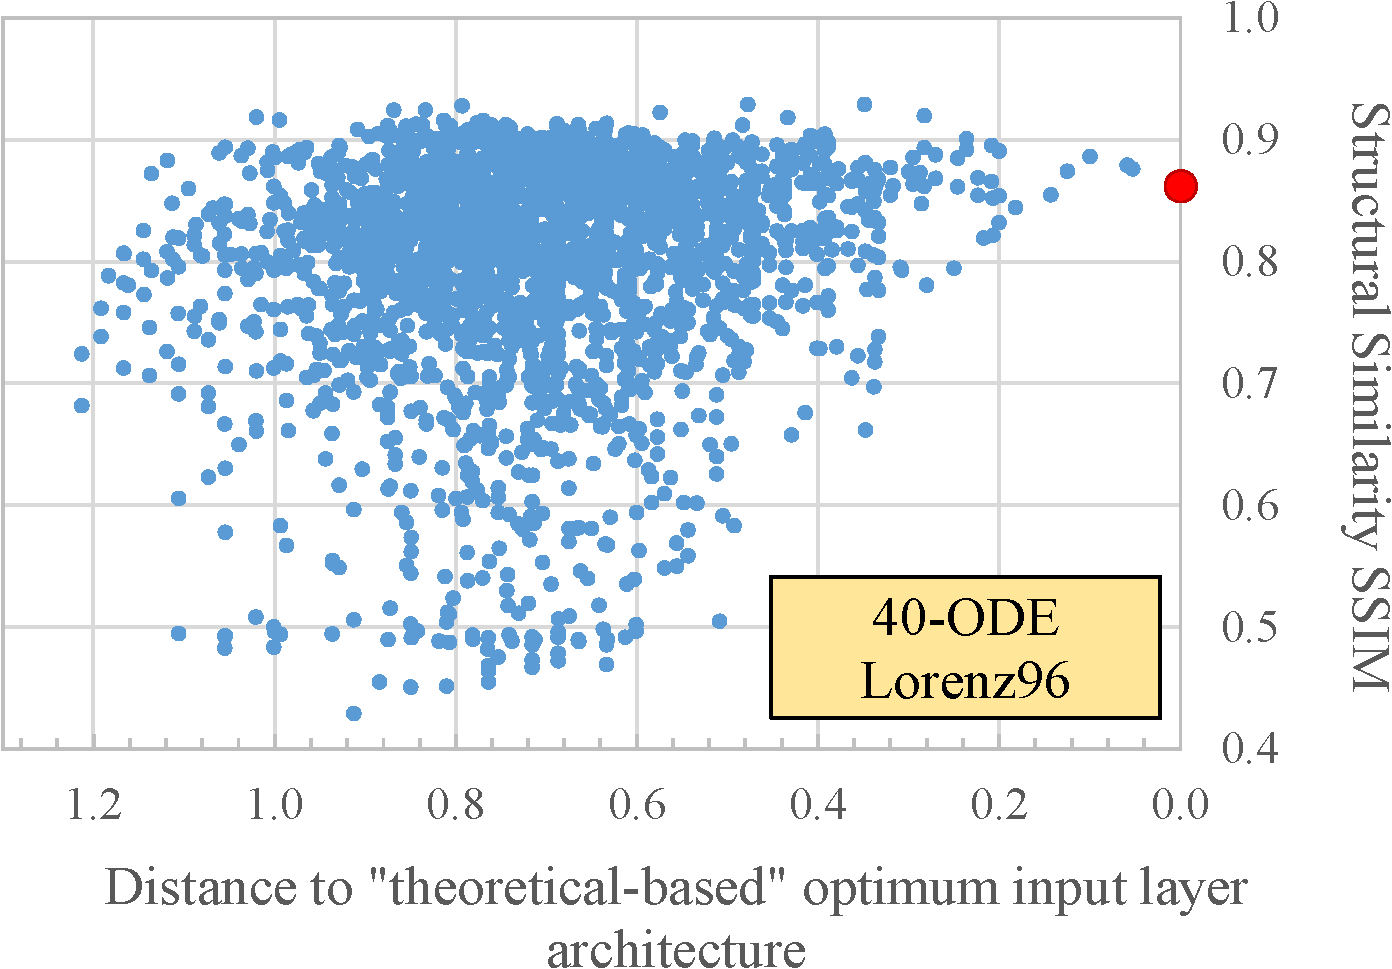
\includegraphics[]{MonteCarloSSIMversusParameterMetricDistanceLorenz96-crop.pdf}}
\caption{Monte Carlo simulation of different  input representations of the input layer for the neural network forecast for the 40-ODE Lorenz 96 system.
It shows the structural similarity (SSIM) against how far (in a Euclidean space metric) the particular parameters of a particular
run was from the supposedly optimal input representation parameters (red dot). The green line (trendline) seems to show that as the parameters
of a randomly chosen input representation get close to the supposedly optimal input representation ones, the SSIM converges to what seems to be the
best possible forecast value given the limited (and noisy) dataset.}
% https://en.wikipedia.org/wiki/Lorenz_96_model
\label{MonteCarloSSIMversusParameterMetricDistanceLorenz96}
\end{figure}

% code in
% C:\Users\eurico\SunspotAnalysis\SpatialTemporalFeatureSelectionOptimalApproach\lorenz4D\lorenz4Drun.m
%%% the Lorenz model is: (cyclical)
% dX[j]/dt=(X[j+1]-X[j-2])*X[j-1]-X[j]+F
%J=40;               %the number of variables
%h=0.05;             %the time step
% results in
% C:\Users\eurico\SunspotAnalysis\SpatialTemporalFeatureSelectionOptimalApproach\KuramotoSivashinsky23_Lorenz.xlsm

For the spatially extended coupled ODEs model we used a well-known 40-coupled ODE dynamical system proposed by Edward Lorenz in 1996 
\cite{articleLorenz96}:

\begin{equation}
\label{lorenz96equations}
\frac{dx_j}{dt}=\left( x_{j+1} - x_{j-2} \right ) x_{j-1} - x_j + F, \, j=1,\ldots,N=40,
\end{equation}
where $x_{-1}=x_{N-1}$, $x_0=x_N$ and $x_{N+1}=x_1$ and $F$ is a forcing term. 
We use the forcing $F=5$ to get some interesting behaviour in space and time. We used a time step $\Delta t=0.05$ and 
we have integrated this equation using J.\ Amezcua's MATLAB code as given in \cite{BibEntry2018Apr}. It uses the 
Runge-Kutta 4-step method.



We run the synthetic data generation for $N=531$ time steps, and divided the set into $N_{\textnormal{train}}=500$ time steps for the training set
and $N_{\textnormal{test}}=31$ time steps for the test set. The other parameters of the neural network were:
$N_h=10$, $\eta=0.05$, $\alpha=0.001$, a linear normalization input scaling with $\alpha_{nor} = 10$ and $\beta_{nor} = 0.430$, 
weight initialization with $\alpha_{rng} = 10^{-3}$ and $\beta_{rng} = -0.5$ and $N_{\textnormal{steps}}=100,000$. 
We used the ReLU function as the activation on both the hidden and output layers.

For this case the optimal values obtained before the Monte Carlo simulation from the mutual information and false neighbours methods 
were $I^*=2$, $J^*=2$, $K^*=1$ and $L^*=9$. The results of the random sampling of $I$, $J$, $K$, $L$ in the simulation
are depicted in Fig.\ \ref{MonteCarloSSIMversusParameterMetricDistanceLorenz96}.  It shows a dispersion as conjectured and a quite a good
convergence to the highest 
$\textnormal{SSIM}$ value we could obtain for this particular slicing of the training and forecast sets: $\textnormal{SSIM}=
0.861844038$. Results seems to suggest the same structure as depicted in our conjecture diagram and in the previous results for sunspots
and the coupled H\'{e}non maps.

\subsection{Partial Differential Equations - Kuramoto-Sivashinsky model}

\begin{figure}[!htb]
\centering
\resizebox{\hsize}{!}{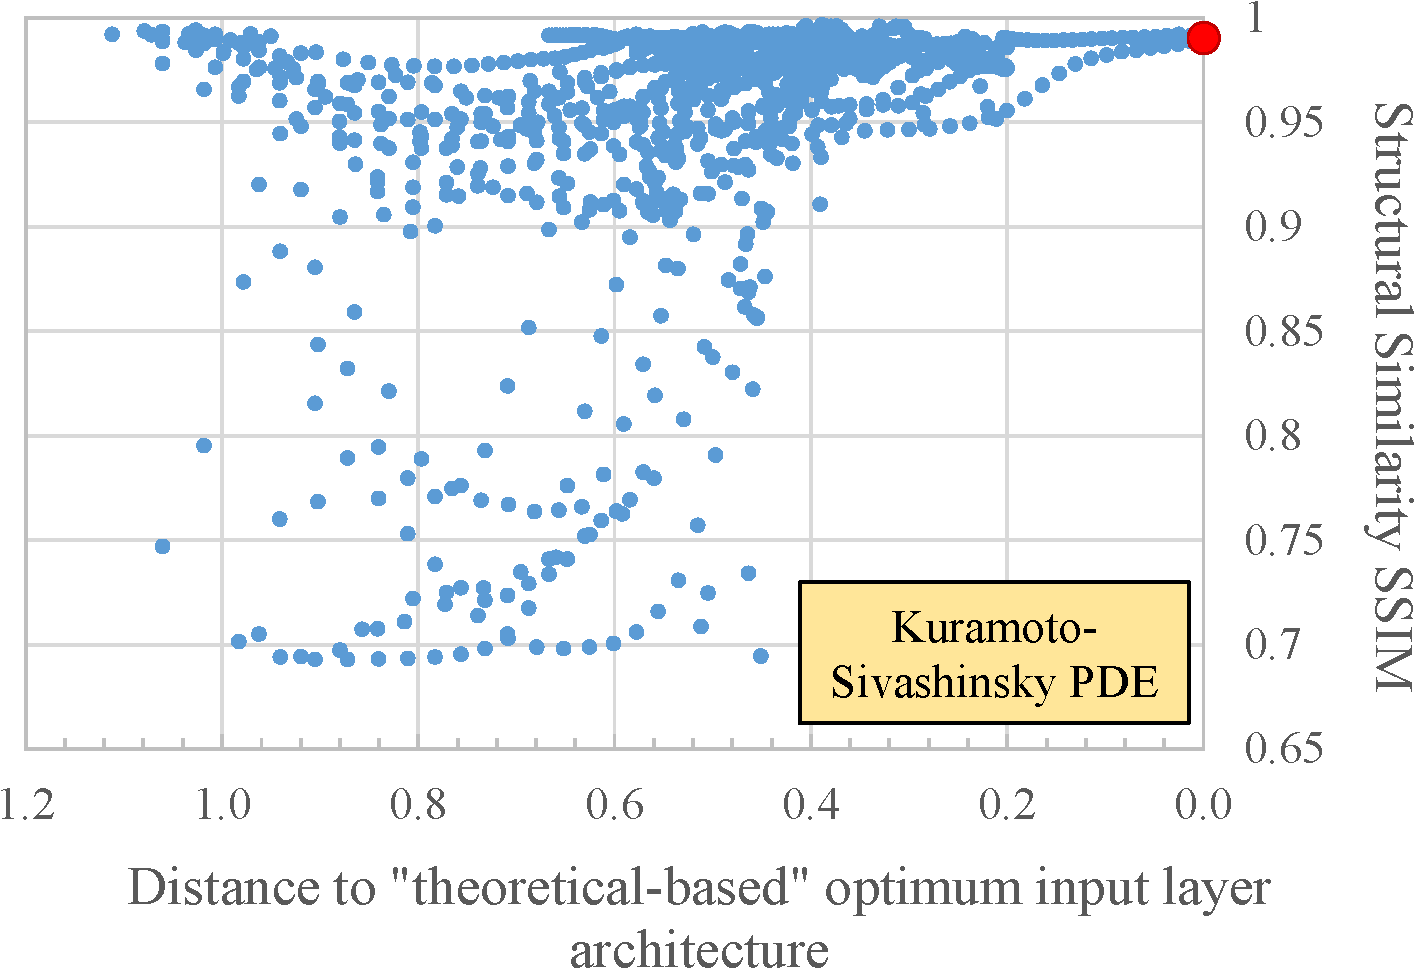
\includegraphics[]{MonteCarloSSIMversusParameterMetricDistanceKS_L=22-crop.pdf}}
\caption{Monte Carlo simulation of different  input representations of the input layer for the neural network forecast for
Kuramoto-Sivashinsky with $L=22$ system.
It shows the structural similarity (SSIM) against how far (in a Euclidean space metric) the particular parameters of a particular
run was from the supposedly optimal input representation parameters (red dot). The green line (trendline) seems to show that as the parameters
of a randomly chosen input representation get close to the supposedly optimal input representation ones, the SSIM converges to what seems to be the
best possible forecast value given the limited (and noisy) dataset.}
\label{MonteCarloSSIMversusParameterMetricDistanceKS_L=22}
\end{figure}

% code in
% C:\Users\eurico\SunspotAnalysis\SpatialTemporalFeatureSelectionOptimalApproach\KSEproject\matlabKSintrinsicSolver.m
% from http://chaosbook.org/extras/KSEproject/html/index.html
% results in
% C:\Users\eurico\SunspotAnalysis\SpatialTemporalFeatureSelectionOptimalApproach\KuramotoSivashinsky28.xlsm

Finally we take a full PDE system, the Kuramoto-Sivashinsky model \cite{1976PThPh..55..356K,1977AcAau...4.1177S},
a very well-known system capable of spatial-temporal chaos
and complex spatial-temporal dynamics. It is a fourth-order nonlinear PDE introduced in the 1970s by Yoshiki
Kuramoto and Gregory Sivashinsky to model the diffusive instabilities
in a laminar flame front.
The model is described by the following equation:

\begin{equation}
\label{kuramotoSivashinskyequation}
\frac{\partial u(x,t)}{\partial t} = -\frac{\partial^4 u(x,t)}{\partial x^4}-\frac{\partial^2 u(x,t)}{\partial x^2}-u(x,t)
\frac{\partial u(x,t)}{\partial x},
\end{equation}
where $x \in [-\frac{L}{2},+\frac{L}{2}]$ with a period boundary condition 
$u(x+L,t)=u(x,t)$. The nature of solutions depends on the system size $L$ and on the initial $u(x,t=0)$. 
We have integrated this equation by taking an exponential time difference Runge-Kutta 4th order method (ETDRK4)
using the Matlab code by P.\ Cvitanovi\'c as given in \cite{BibEntry2007Apr} and 
taking a time step of $\Delta t=0.5$, $L=22$ Fourier modes which are known to produce a ``turbulent'' or chaotic behaviour
and a initial condition $u(x,t=0)=10^{-5}$ for $x\in[5,15]$, the remain being $u(x,t=0)=0$.



We run the simulation for $N=531$ time steps, and divided the set into $N_{\textnormal{train}}=500$ time steps for the training set
and $N_{\textnormal{test}}=31$ time steps for the test set. The other parameters of the neural network were:
$N_h=50$, $\eta=0.1$, $\alpha=0$, a linear normalization input scaling with 
$\alpha_{nor} = 5.8472$ and $\beta_{nor} =0.5$, weight initialization 
with $\alpha_{rng} = 10^{-3}$ and $\beta_{rng} = -0.5$ and $N_{\textnormal{steps}}=$\SI{1000000}\nobreak. 
We used the ReLU function as the activation on both the hidden and output layers.

The results of the Monte Carlo simulation can be seen in Fig.\ \ref{MonteCarloSSIMversusParameterMetricDistanceKS_L=22}. For this 
case the optimal values obtained before we run the Monte Carlo simulation were $I^*=1$, $J^*=2$, $K^*=2$ and $L^*=39$. It again shows a dispersion as 
conjectured and a excellent convergence to the highest $\textnormal{SSIM}$ value we could obtain for this particular slicing of the training and 
test sets: a surprising high value of $\textnormal{SSIM}=0.990264382$. Results seems to suggest the same structure as depicted in our 
conjecture diagram and in the previous results for sunspots, the coupled H\'{e}non maps and coupled ODEs. 


% Note that the IEEE typically puts floats only at the top, even when this
% results in a large percentage of a column being occupied by floats.


% An example of a double column floating figure using two subfigures.
% (The subfig.sty package must be loaded for this to work.)
% The subfigure \label commands are set within each subfloat command,
% and the \label for the overall figure must come after \caption.
% \hfil is used as a separator to get equal spacing.
% Watch out that the combined width of all the subfigures on a
% line do not exceed the text width or a line break will occur.
%
%\begin{figure*}[!t]
%\centering
%\subfloat[Case I]{\includegraphics[width=2.5in]{box}%
%\label{fig_first_case}}
%\hfil
%\subfloat[Case II]{\includegraphics[width=2.5in]{box}%
%\label{fig_second_case}}
%\caption{Simulation results for the network.}
%\label{fig_sim}
%\end{figure*}
%
% Note that often IEEE papers with subfigures do not employ subfigure
% captions (using the optional argument to \subfloat[]), but instead will
% reference/describe all of them (a), (b), etc., within the main caption.
% Be aware that for subfig.sty to generate the (a), (b), etc., subfigure
% labels, the optional argument to \subfloat must be present. If a
% subcaption is not desired, just leave its contents blank,
% e.g., \subfloat[].


% An example of a floating table. Note that, for IEEE style tables, the
% \caption command should come BEFORE the table and, given that table
% captions serve much like titles, are usually capitalized except for words
% such as a, an, and, as, at, but, by, for, in, nor, of, on, or, the, to
% and up, which are usually not capitalized unless they are the first or
% last word of the caption. Table text will default to \footnotesize as
% the IEEE normally uses this smaller font for tables.
% The \label must come after \caption as always.
%
%\begin{table}[!t]
%% increase table row spacing, adjust to taste
%\renewcommand{\arraystretch}{1.3}
% if using array.sty, it might be a good idea to tweak the value of
% \extrarowheight as needed to properly center the text within the cells
%\caption{An Example of a Table}
%\label{table_example}
%\centering
%% Some packages, such as MDW tools, offer better commands for making tables
%% than the plain LaTeX2e tabular which is used here.
%\begin{tabular}{|c||c|}
%\hline
%One & Two\\
%\hline
%Three & Four\\
%\hline
%\end{tabular}
%\end{table}


% Note that the IEEE does not put floats in the very first column
% - or typically anywhere on the first page for that matter. Also,
% in-text middle ("here") positioning is typically not used, but it
% is allowed and encouraged for Computer Society conferences (but
% not Computer Society journals). Most IEEE journals/conferences use
% top floats exclusively.
% Note that, LaTeX2e, unlike IEEE journals/conferences, places
% footnotes above bottom floats. This can be corrected via the
% \fnbelowfloat command of the stfloats package.




\section{Conclusion}
\label{conclusionsection}
We have shown empirical evidence for the existence of an optimal feature selection for the input layer of feedforward neural networks used to 
forecast spatial-temporal series. We believe that the selection of the features of the input layer can be uniquely determined by 
the data itself, using two techniques from dynamical systems embedding theory: the mutual information and the false neighbours 
methods. The former procedure determines the temporal and spatial delays to take when selecting features, while the latter  
determines the number of data points in space and time to be taken as inputs.  We conjecture that this optimal feature selection gives the best 
forecast, as measured by a standard image similarity index. We also conjecture that the shape of the dispersion of points on a Monte Carlo 
simulation across all possible feature selections on a plot of the similarity index versus the 
distance to optimal feature selection is a skewed bell  
shape with the highest value being the optimal feature selection/maximum similarity index.
  
In order to substantiate our conjecture, we choose four unrelated systems, in order of complexity: a set of spatially 
extended coupled maps; a set of spatially extended coupled ODEs; a one-dimensional spatial PDE and a real spatial-temporal data set from 
sunspots areas in our Sun. In all four cases, we were able to first use the mutual information and the false neighbours methods to 
determine the four parameters defining the input layer feature selection\footnote{We have four parameters for the feature selection 
in these cases, with one temporal and one spatial dimension. For higher dimensional systems, there will be more parameters, the exact 
number being double the number of dimensions of the system.}. After calibration of the hyperparameters we then were able to forecast 
reasonably the test set, although this is not the objective or primary goal of this article. 
We then show that for a random Monte Carlo simulation across possible feature selections, the neural network did not, 
as expected, forecast as well as it did for the specific set of optimal four parameters given by dynamical systems theory. As conjectured, the Monte Carlo 
simulations show that the shape of the distribution of points was a 
skewed bell shape with the highest value being the optimal feature selection/maximum similarity index (subject to minor variations due to noise
and the finiteness of the dataset).

Given how important spatial-temporal systems are 
and how we want to forecast the future as accurately as possible 
it is quite 
important to attempt to reduce the number of hyperparameters in neural network prediction, and to try to constraint the feature selection from 
the data properties only. If indeed our conjecture turns out to be true, it would remove the input layer feature selection as another free 
parameter in the already complex process of choosing the details of the neural network to use for forecasting.

In this article we have focused first and foremost in establishing empirical evidence for our conjecture, within a simple framework of 
feedforward neural networks with one hidden layer for the purpose of prediction in one spatial and one temporal dimensions. Naturally, 
there are many clear extensions to our research. First to use deeper networks with more hidden 
layers to possible tackle systems which are hyperchaotic (i.e. with multiple positive Lyapunov exponents). Second, to attempt to extend the conjecture with empirical evidence in high 
dimensions, e.g. 3+1-dimensional weather systems. Third, to extend the conjecture to more complex and fashionable
neural networks models, such as recurrent neural networks, particularly echo state networks and long short-term memory networks.
 Fourth and last but not least, to prove the conjecture would show how dynamical systems theory can clarify the so call
 ``dark arts'' in neural network feature construction. These objectives are however, outside the scope
 of this research article and will be pursued later.

% if have a single appendix:
%\appendix[Proof of the Zonklar Equations]
% or
%\appendix  % for no appendix heading
% do not use \section anymore after \appendix, only \section*
% is possibly needed

% use appendices with more than one appendix
% then use \section to start each appendix
% you must declare a \section before using any
% \subsection or using \label (\appendices by itself
% starts a section numbered zero.)
%


%\appendices
%\section{Proof of the First Zonklar Equation}
%Appendix one text goes here.

% you can choose not to have a title for an appendix
% if you want by leaving the argument blank
%\section{}
%Appendix two text goes here.


% use section* for acknowledgment
\section*{Acknowledgment}
We would like to thank Prof. Reza Tavakol from Queen Mary University London for very useful discussions on forecasting. We also thank
Dr.\ David Hathaway from NASA's Ames Research Centre for providing the sunspot data on which some of the results in this article are based upon.
CITEUC is funded by National Funds through FCT - Foundation for Science
and Technology (project: UID/Multi/00611/2013) and FEDER - European
Regional Development Fund through
COMPETE 2020 - Operational Programme Competitiveness and
Internationalization (project: POCI-01-0145-FEDER-006922).

% Can use something like this to put references on a page
% by themselves when using endfloat and the captionsoff option.
\ifCLASSOPTIONcaptionsoff
  \newpage
\fi

% trigger a \newpage just before the given reference
% number - used to balance the columns on the last page
% adjust value as needed - may need to be readjusted if
% the document is modified later
%\IEEEtriggeratref{8}
% The "triggered" command can be changed if desired:
%\IEEEtriggercmd{\enlargethispage{-5in}}

% references section

\newcommand*\aap{A\&A}
\let\astap=\aap
\newcommand*\aapr{A\&A~Rev.}
\newcommand*\aaps{A\&AS}
\newcommand*\actaa{Acta Astron.}
\newcommand*\aj{AJ}
\newcommand*\ao{Appl.~Opt.}
\let\applopt\ao
\newcommand*\apj{ApJ}
\newcommand*\apjl{ApJ}
\let\apjlett\apjl
\newcommand*\apjs{ApJS}
\let\apjsupp\apjs
\newcommand*\aplett{Astrophys.~Lett.}
\newcommand*\apspr{Astrophys.~Space~Phys.~Res.}
\newcommand*\apss{Ap\&SS}
\newcommand*\araa{ARA\&A}
\newcommand*\azh{AZh}
\newcommand*\baas{BAAS}
\newcommand*\bac{Bull. astr. Inst. Czechosl.}
\newcommand*\bain{Bull.~Astron.~Inst.~Netherlands}
\newcommand*\caa{Chinese Astron. Astrophys.}
\newcommand*\cjaa{Chinese J. Astron. Astrophys.}
\newcommand*\fcp{Fund.~Cosmic~Phys.}
\newcommand*\gca{Geochim.~Cosmochim.~Acta}
\newcommand*\grl{Geophys.~Res.~Lett.}
\newcommand*\iaucirc{IAU~Circ.}
\newcommand*\icarus{Icarus}
\newcommand*\jcap{J. Cosmology Astropart. Phys.}
\newcommand*\jcp{J.~Chem.~Phys.}
\newcommand*\jgr{J.~Geophys.~Res.}
\newcommand*\jqsrt{J.~Quant.~Spec.~Radiat.~Transf.}
\newcommand*\jrasc{JRASC}
\newcommand*\memras{MmRAS}
\newcommand*\memsai{Mem.~Soc.~Astron.~Italiana}
\newcommand*\mnras{MNRAS}
\newcommand*\na{New A}
\newcommand*\nar{New A Rev.}
\newcommand*\nat{Nature}
\newcommand*\nphysa{Nucl.~Phys.~A}
\newcommand*\pasa{PASA}
\newcommand*\pasj{PASJ}
\newcommand*\pasp{PASP}
\newcommand*\physrep{Phys.~Rep.}
\newcommand*\physscr{Phys.~Scr}
\newcommand*\planss{Planet.~Space~Sci.}
\newcommand*\pra{Phys.~Rev.~A}
\newcommand*\prb{Phys.~Rev.~B}
\newcommand*\prc{Phys.~Rev.~C}
\newcommand*\prd{Phys.~Rev.~D}
\newcommand*\pre{Phys.~Rev.~E}
\newcommand*\prl{Phys.~Rev.~Lett.}
\newcommand*\procspie{Proc.~SPIE}
\newcommand*\qjras{QJRAS}
\newcommand*\rmxaa{Rev. Mexicana Astron. Astrofis.}
\newcommand*\skytel{S\&T}
\newcommand*\solphys{Sol.~Phys.}
\newcommand*\sovast{Soviet~Ast.}
\newcommand*\ssr{Space~Sci.~Rev.}
\newcommand*\zap{ZAp}

% can use a bibliography generated by BibTeX as a .bbl file
% BibTeX documentation can be easily obtained at:
% http://mirror.ctan.org/biblio/bibtex/contrib/doc/
% The IEEEtran BibTeX style support page is at:
% http://www.michaelshell.org/tex/ieeetran/bibtex/
%\bibliographystyle{IEEEtran}
% argument is your BibTeX string definitions and bibliography database(s)
%\bibliography{IEEEabrv,../bib/paper}
\bibliographystyle{IEEEtran}
%\bibliography{IEEEabrv,eurico} % your references Yourfile.bib
\bibliography{eurico} % your references Yourfile.bib
%
% <OR> manually copy in the resultant .bbl file
% set second argument of \begin to the number of references
% (used to reserve space for the reference number labels box)
%\begin{thebibliography}{1}

%\bibitem{IEEEhowto:kopka}
%H.~Kopka and P.~W. Daly, \emph{A Guide to \LaTeX}, 3rd~ed.\hskip 1em plus
%  0.5em minus 0.4em\relax Harlow, England: Addison-Wesley, 1999.

%\end{thebibliography}

% biography section
%
% If you have an EPS/PDF photo (graphicx package needed) extra braces are
% needed around the contents of the optional argument to biography to prevent
% the LaTeX parser from getting confused when it sees the complicated
% \includegraphics command within an optional argument. (You could create
% your own custom macro containing the \includegraphics command to make things
% simpler here.)
%\begin{IEEEbiography}[{\includegraphics[width=1in,height=1.25in,clip,keepaspectratio]{mshell}}]{Eurico Covas}
% or if you just want to reserve a space for a photo:

\begin{IEEEbiographynophoto}{Eurico Covas}
Biography text here.
\end{IEEEbiographynophoto}

% if you will not have a photo at all:
\begin{IEEEbiographynophoto}{Emmanouil Benetos}
Biography text here.
\end{IEEEbiographynophoto}

% insert where needed to balance the two columns on the last page with
% biographies
%\newpage

% You can push biographies down or up by placing
% a \vfill before or after them. The appropriate
% use of \vfill depends on what kind of text is
% on the last page and whether or not the columns
% are being equalized.

%\vfill

% Can be used to pull up biographies so that the bottom of the last one
% is flush with the other column.
%\enlargethispage{-5in}



% that's all folks
\end{document}


